\FloatBarrier
\section{Rolling Adapter Admission Frequencies}\label{app:rolling-admissions}

\Cref{fig:fw-rolling-admissions} uses a separate recent capture of adapter
decisions. The earlier ledger in \cref{tab:admission-ledger} retains its
own capture and cutoff. Each trailing window contains exactly 100 observed
decisions, including accepted ties and rejected candidates. These overlapping
counts describe the logged policy on an adaptively reused development
population; the independent first-proposal comparison remains pending.

\begin{figure}[htb]
  \centering
  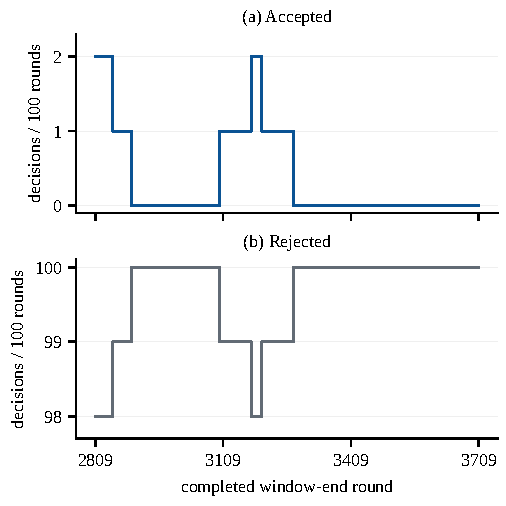
\includegraphics[width=\linewidth]{figures/fig_fw_rolling_admissions.pdf}
  \caption{\textbf{Trailing 100-round adapter acceptance and rejection counts.}
  The source window contains \num{1000} consecutive completed rounds,
  2710--3709, captured at 13:30 UTC on 2 November 2026. It records four
  admissions (two strict gains and two exact ties) and 996 rejections.
  Panels (a) and (b) show the complementary accepted and rejected counts
  in each full trailing window, plotted at its final round: 2809--3709,
  or 901 overlapping windows. The first 99 source rows supply history
  without a plotted partial window. Every accepted/rejected pair sums to
  100; one decision per 100 rounds also equals one percentage point.
  Decisions use unrounded candidate and prior-best utility.
  These are adapter admissions, distinct from training-program incumbent
  events; no uncertainty interval or independent improvement estimate is
  implied. Scope: \cref{sec:method-status}.}
  \label{fig:fw-rolling-admissions}
\end{figure}
\subsection{Recorded selection changes}\label{app:selection-changes}

The observer in \cref{fig:fw-selection-changes} refuses changed evaluation
identities, inconsistent selection counts and duplicate context identifiers
before comparing ordered program identities. It counts candidate and retained
differences from one stored reference, rather than utility changes.
The tie-admission and best-round identity rules follow
\cref{sec:method-status}.
These changes occur on reused development contexts; matched controls are
still required for \mbox{attribution to training} or proposal quality.

\begin{figure}[htbp]
  \centering
  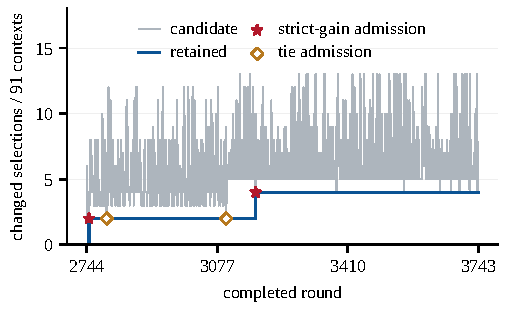
\includegraphics[width=\linewidth]{figures/fig_fw_selection_changes.pdf}
  \caption{\textbf{Retained program selections change only at admitted rounds.}
  Rounds 2744--3743, captured at 14:34 UTC on 2 November 2026.
  All \num{1000} completed records compare selections on 91 reused
  development contexts with the recorded round-882 reference.
  Grey: candidate before admission; blue: post-decision retained selections.
  Stars: two strict-gain admissions; hollow diamonds: two accepted ties;
  the other 996 decisions are rejections. These descriptive identity
  counts do not establish a training effect, writer or ranking-map benefit,
  or independent proposal quality. Scope: \cref{sec:method-status}.}
  \label{fig:fw-selection-changes}
\end{figure}

